\documentclass{ieeeaccess}
\usepackage{cite}
\usepackage{amsmath,amssymb,amsfonts}
\usepackage{algorithm,algorithmic}
\usepackage{graphicx}
\usepackage{textcomp}
\usepackage{bm}
\usepackage{float}
\makeatletter
\AtBeginDocument{\DeclareMathVersion{bold}
    \SetSymbolFont{operators}{bold}{T1}{times}{b}{n}
    \SetSymbolFont{NewLetters}{bold}{T1}{times}{b}{it}
    \SetMathAlphabet{\mathrm}{bold}{T1}{times}{b}{n}
    \SetMathAlphabet{\mathit}{bold}{T1}{times}{b}{it}
    \SetMathAlphabet{\mathbf}{bold}{T1}{times}{b}{n}
    \SetMathAlphabet{\mathtt}{bold}{OT1}{pcr}{b}{n}
    \SetSymbolFont{symbols}{bold}{OMS}{cmsy}{b}{n}
    \renewcommand\boldmath{\@nomath\boldmath\mathversion{bold}}}
\makeatother

\def\BibTeX{{\rm B\kern-.05em{\sc i\kern-.025em b}\kern-.08em
T\kern-.1667em\lower.7ex\hbox{E}\kern-.125emX}}

%Your document starts from here ___________________________________________________
\begin{document}
\history{Date of publication xxxx 00, 0000, date of current version xxxx 00,
    0000.}
\doi{10.1109/ACCESS.2024.0429000}

\title{Vega: A Chatbot Platform for Development of Internet of Things}
% //TODO: ask about IEEE membership
\author{\uppercase{Harith Al-Safi}, \IEEEmembership{Fellow, IEEE},
    \uppercase{Harith Ibrahim}, and Paul Steenson,
    \IEEEmembership{SeniroMember, IEEE}}

\address{School of Electronics and Electrical Engineering, University of Leeds,
    Leeds LS2 9JT, U.K}
\tfootnote{This paragraph of the first footnote will contain support
    information, including sponsor and financial support acknowledgment. For
    example, ``This work was supported in part by the U.S. Department of
    Commerce under Grant BS123456.''}

\markboth
{Author \headeretal: Preparation of Papers for IEEE TRANSACTIONS and JOURNALS}
{Author \headeretal: Preparation of Papers for IEEE TRANSACTIONS and JOURNALS}

\corresp{Corresponding author: Harith Al-Safi (e-mail:
    harith.alsafi@gmail.com).}

\begin{abstract}
    Large language models (LLMs) have revolutionized natural language
    processing, yet their potential in Internet of Things (IoT) applications
    remains largely untapped. Traditional IoT interfaces often require specialized
    knowledge, creating barriers for non-technical users. We present a modular
    system that leverages LLMs to enable intuitive, natural language control of IoT
    devices, specifically a Raspberry Pi (RPi) connected to various sensors and
    devices. Our solution comprises three key components: a physical circuit with
    input and output devices, an RPi integrating Control Server, and a web
    application integrating LLM logic. Users interact with the system through
    natural language commands, which the LLM interprets to call appropriate
    commands for the RPi. The RPi executes these instructions on the connected
    circuit, with outcomes communicated back to the user via LLM-generated
    responses. We empirically evaluate our system's performance across a range of
    task complexities and user scenarios, demonstrating its ability to handle
    complex, conditional logic without additional RPi-level coding. Our findings
    reveal that LLM-driven IoT control can effectively bridge the gap between
    complex device functionality and user-friendly interaction. We discuss the
    system's scalability, exploring its potential applications in diverse settings
    such as smart homes, industrial monitoring, and educational environments. By
    enabling natural language interaction with IoT devices, our approach not only
    enhances accessibility for non-technical users but also opens new avenues for
    creative and intelligent IoT applications. This research contributes to the
    growing body of work on interactive intelligent systems for IoT, offering
    insights into the design and implementation of LLM-integrated IoT interfaces.
\end{abstract}

\begin{keywords}
    Enter key words or phrases in alphabetical
    order, separated by commas. Autocorrelation, beamforming, communications
    technology, dictionary learning, feedback, fMRI, mmWave, multipath, system
    design, multipath, slight fault, underlubrication fault.
\end{keywords}

\titlepgskip=-21pt

\maketitle

\section{Introduction}
\label{sec:introduction}
\PARstart{T}{he} evolution of large language models (LLM's) has led to rapid
development in the  realm of intelligent systems. However, the application of
LLM's hasn't been thoroughly explored in internet of things (IoT) and embedded
systems (ESys). Traditionally, the development of IoT systems that seamlessly
adapt to the user's need and tasks poses a considerable challenge. Leveraging
the capabilities of LLMs presents an opportunity to address this challenge and
bridge the gap between technical intricacies and user accessibility.
\section{Background and Related Work}

\subsection{ProgPrompt}
\subsection{ToD4IR}
\subsection{CASIT}

% \Figure[t!](topskip=0pt, botskip=0pt, midskip=0pt)[width=\textwidth]{{figures/fig1.png}}
% { \textbf{Magnetization as a function of applied field.
% It is good practice to explain the significance of the figure in the caption.}\label{fig1}}

\section{Methodology}

\subsection{Overall Architecture}
\Figure[t!](topskip=0pt, botskip=0pt,
midskip=0pt)[width=\textwidth]{{figures/fig2.png}}
{ \textbf{The overall arhcitecture of the system.}\label{fig1}}
A
% \begin{table}
%     \caption{\textbf{Units for Magnetic Properties}}
%     \label{table}
%     \setlength{\tabcolsep}{2pt}
%     \begin{tabular}{|p{65pt}|p{35pt}|p{45pt}|p{75pt}|}
%     \hline
%     Module Name&
%     Language&
%     Framework&
%     Main Libraries \\
%     \hline
%     Webapp interface&
%     Typescript&
%     React.js&
%     RadixUI,TailwindCSS\\
%     Webapp logic&
%     Typescript&
%     Next.js, Node.js&
%     OpenAI\\
%     \hline

%     \end{tabular}
%     \label{tab1}
%     \end{table}

\subsection{Physical Circuit Design}

\Figure[t!](topskip=0pt, botskip=0pt,
midskip=0pt)[width=\textwidth]{{figures/fig5.png}}
{ \textbf{Soldered physical circuit connected to the RPi}\label{fig1}}

\subsection{Raspberry Pi Design}
\begin{table}
    \caption{\textbf{Physical devices defined on the Control Server, which are then supplied to the LLM}}
    \label{table1}
    \setlength{\tabcolsep}{3pt}
    \begin{tabular}{|p{30pt}|p{25pt}|p{180pt}|}
        \hline
        \textbf{Symbol} &
        \textbf{Type}   &
        \textbf{Description}                                             \\
        \hline
        ULTS   &
        Input  &
        Ultrasonic Distance Sensor in 'cm'                      \\
        \hline
        CAM    &
        Input  &
        Camera device for picture input                         \\
        \hline
        GPS    &
        Input  &
        GPS device for longitude and latitude coordinates       \\
        \hline
        TMP    &
        Input  &
        Temperature sensor giving response in degree celcuis    \\
        \hline
        FAN    &
        Output &
        12V fan controled by a digital GPIO pin through a relay \\
        \hline
        LCD    &
        Output &
        I2C LCD for displaying strings                          \\
        \hline
        SRV    &
        Output &
        Servo motor rotates using PWM to a given angles         \\
        \hline
        LED1   &
        Output &
        Yellow LED light                                        \\
        \hline
        LED2   &
        Output &
        Red LED light                                           \\
        \hline
        LED3   &
        Output &
        Blue LED light                                          \\
        \hline
    \end{tabular}
\end{table}

\begin{table}
    \caption{\textbf{Defined functions on the Control Server, called by the LLM based on user input, executes on the RPi and processed on the webapp}}
    \label{table2}
    \setlength{\tabcolsep}{3pt}
    \begin{tabular}{|p{80pt}|p{70pt}|p{85pt}|}
        \hline
        \textbf{Function}    &
        \textbf{Description} &
        \textbf{Use Case} \\
        \hline
        set\underbar{ }led   &
        Toggles specefic LED &
        "Turn on yellow LED" \\
        \hline 
        set\underbar{ }fan   &
        Toggles fan on or off &
        "Turn on the fan" \\
        \hline
        get\underbar{ }recorded\underbar{ }sensor\underbar{ }data   &
        Gets interval sensor data from database &
        "Plot me the distance data in last 30 seconds" \\
        \hline
        get\underbar{ }raspberry\underbar{ }stats   &
        Gets CPU, RAM, Disk of RPi&
        "What is the currrent disk usage" \\
        \hline
        capture\underbar{ }image   &
        Captures an image and uploads it to Imgur &
        "Capture an image, does it contain a pen?" \\
        \hline
        get\underbar{ }connected\underbar{ }devices    &
        Fetches the data of connected devices &
        "What is the current humidity and temperature" \\
        \hline
        get\underbar{ }location\underbar{ }   &
        Gets the current location from GPS&
        "From the location are we currently in Leeds?" \\
        \hline
        set\underbar{ }servo\underbar{ }angles    &
        Turn servo to certain angle &
        "Turn the servo to 10 then 180 degrees" \\
        \hline
    \end{tabular}
\end{table}
\Figure[t!](topskip=0pt, botskip=0pt,
midskip=0pt)[scale=0.40]{{figures/fig6.png}}
{ \textbf{Architecture design of the RPi control server}\label{fig2}}

\subsection{Web App Design}
\Figure[t!](topskip=0pt, botskip=0pt,
midskip=0pt)[width=\textwidth]{{figures/fig9.png}}
{ \textbf{Webapp user interface implementation}\label{fig3}}
\Figure[t!](topskip=0pt, botskip=0pt,
midskip=0pt)[width=\textwidth]{{figures/fig13.png}}
{ \textbf{Webapp logic design}\label{fig4}}

\section{Experiment and Results}
\label{sec:guidelines}

\subsection{Complex Commands}
\Figure[t!](topskip=0pt, botskip=0pt,
midskip=0pt)[width=\textwidth]{{figures/fig30.png}}
{ \textbf{System case studies}\label{fig5}}


\subsection{Automated Evaluation}
% \Figure[t!](topskip=0pt, botskip=0pt, midskip=0pt)[width=\textwidth]{{figures/fig15.png}}
% { \textbf{Magnetization as a function of applied field.
% It is good practice to explain the significance of the figure in the caption.}\label{fig6}}
\subsection{Result Analysis}
\Figure[t!](topskip=0pt, botskip=0pt,
midskip=0pt)[width=0.99\columnwidth]{{figures/fig17.png}}
{ \textbf{Magnetization as a function of applied field.
        It is good practice to explain the significance of the figure in the
        caption.}\label{fig6}}
\Figure[t!](topskip=0pt, botskip=0pt,
midskip=0pt)[width=0.99\columnwidth]{{figures/fig18.png}}
{ \textbf{Magnetization as a function of applied field.
        It is good practice}\label{fig7}}
\Figure[t!](topskip=0pt, botskip=0pt,
midskip=0pt)[width=0.99\columnwidth]{{figures/fig19.png}}
{ \textbf{Magnetization as a function of applied field.
        It is good practice}\label{fig8}}
% \Figure[t!](topskip=0pt, botskip=0pt,
% midskip=0pt)[width=0.99\columnwidth]{{figures/fig26.png}}
% { \textbf{Magnetization as a function of applied field.
%         It is good practice to explain the significance of the figure in the
%         caption.}\label{fig9}}
\Figure[t!](topskip=0pt, botskip=0pt,
midskip=0pt)[width=0.99\columnwidth]{{figures/fig32.png}}
{ \textbf{Magnetization as a function of applied field.
        It is good practice to explain the significance of the figure in the
        caption.}\label{fig9}}

\Figure[t!](topskip=0pt, botskip=0pt,
midskip=0pt)[width=0.99\columnwidth]{{figures/fig33.png}}
{ \textbf{Magnetization as a function of applied field.
        It is good practice to explain the significance of the figure in the
        caption.}\label{fig10}}

\Figure[t!](topskip=0pt, botskip=0pt,
midskip=0pt)[width=0.80\columnwidth]{{figures/fig34.png}}
{ \textbf{Magnetization as a function of applied field.
        It is good practice to explain the significance of the figure in the
        caption.}\label{fig11}}

\Figure[t!](topskip=0pt, botskip=0pt,
midskip=0pt)[width=0.99\columnwidth]{{figures/fig35.png}}
{ \textbf{Magnetization as a function of applied field.
        It is good practice to explain the significance of the figure in the
        caption.}\label{fig12}}


\subsection{Real Life Applicability}

\section{Conclusion}


\section*{Acknowledgment}


\begin{thebibliography}{00}

    \bibitem{b1} G. O. Young, ``Synthetic structure of industrial plastics,''
    in \emph{Plastics,} 2\textsuperscript{nd} ed., vol. 3, J. Peters, Ed. New York,
    NY, USA: McGraw-Hill, 1964, pp. 15--64.

    \bibitem{b2} W.-K. Chen, \emph{Linear Networks and Systems.} Belmont, CA,
    USA: Wadsworth, 1993, pp. 123--135.

    \bibitem{b3} J. U. Duncombe, ``Infrared navigation---Part I: An assessment
    of feasibility,'' \emph{IEEE Trans. Electron Devices}, vol. ED-11, no. 1, pp.
    34--39, Jan. 1959, 10.1109/TED.2016.2628402.

    \bibitem{b4} E. P. Wigner, ``Theory of traveling-wave optical laser,''
    \emph{Phys. Rev}., vol. 134, pp. A635--A646, Dec. 1965.

    \bibitem{b5} E. H. Miller, ``A note on reflector arrays,'' \emph{IEEE
        Trans. Antennas Propagat}., to be published.

    \bibitem{b6} E. E. Reber, R. L. Michell, and C. J. Carter, ``Oxygen
    absorption in the earth's atmosphere,'' Aerospace Corp., Los Angeles, CA, USA,
    Tech. Rep. TR-0200 (4230-46)-3, Nov. 1988.

    \bibitem{b7} J. H. Davis and J. R. Cogdell, ``Calibration program for the
    16-foot antenna,'' Elect. Eng. Res. Lab., Univ. Texas, Austin, TX, USA, Tech.
    Memo. NGL-006-69-3, Nov. 15, 1987.

    \bibitem{b8} \emph{Transmission Systems for Communications},
    3\textsuperscript{rd} ed., Western Electric Co., Winston-Salem, NC, USA, 1985,
    pp. 44--60.

    \bibitem{b9} \emph{Motorola Semiconductor Data Manual}, Motorola
    Semiconductor Products Inc., Phoenix, AZ, USA, 1989.

    \bibitem{b10} G. O. Young, ``Synthetic structure of industrial
    plastics,'' in Plastics, vol. 3, Polymers of Hexadromicon, J. Peters,
    Ed., 2\textsuperscript{nd} ed. New York, NY, USA: McGraw-Hill, 1964, pp.
    15-64.
    [Online]. Available:
    \underline{http://www.bookref.com}.

    \bibitem{b11} \emph{The Founders' Constitution}, Philip B. Kurland
    and Ralph Lerner, eds., Chicago, IL, USA: Univ. Chicago Press, 1987.
        [Online]. Available:
    \underline{http://press-pubs.uchicago.edu/founders/}

    \bibitem{b12} The Terahertz Wave eBook. ZOmega Terahertz Corp., 2014.
        [Online]. Available:
    \underline{http://dl.z-thz.com/eBook/zomegaebookpdf\_1206\_sr.pdf}.
    Accessed on: May 19, 2014.

    \bibitem{b13} Philip B. Kurland and Ralph Lerner, eds., \emph{The
        Founders' Constitution.} Chicago, IL, USA: Univ. of Chicago Press,
    1987, Accessed on: Feb. 28, 2010, [Online] Available:
    \underline{http://press-pubs.uchicago.edu/founders/}

    \bibitem{b14} J. S. Turner, ``New directions in communications,''
    \emph{IEEE J. Sel. Areas Commun}., vol. 13, no. 1, pp. 11-23, Jan. 1995.

    \bibitem{b15} W. P. Risk, G. S. Kino, and H. J. Shaw, ``Fiber-optic
    frequency shifter using a surface acoustic wave incident at an oblique angle,''
    \emph{Opt. Lett.}, vol. 11, no. 2, pp. 115--117, Feb. 1986.

    \bibitem{b16} P. Kopyt \emph{et al., ``}Electric properties of
    graphene-based conductive layers from DC up to terahertz range,'' \emph{IEEE
        THz Sci. Technol.,} to be published. DOI: 10.1109/TTHZ.2016.2544142.

    \bibitem{b17} PROCESS Corporation, Boston, MA, USA. Intranets:
    Internet technologies deployed behind the firewall for corporate
    productivity. Presented at INET96 Annual Meeting. [Online].
    Available: \underline{http://home.process.com/Intranets/wp2.htp}

    \bibitem{b18} R. J. Hijmans and J. van Etten, ``Raster: Geographic analysis
    and modeling with raster data,'' R Package Version 2.0-12, Jan. 12, 2012.
        [Online]. Available: \underline {http://CRAN.R-project.org/package=raster}

    \bibitem{b19} Teralyzer. Lytera UG, Kirchhain, Germany [Online].
    Available:
    \underline{http://www.lytera.de/Terahertz\_THz\_Spectroscopy.php?id=home},
    Accessed on: Jun. 5, 2014.

    \bibitem{b20} U.S. House. 102\textsuperscript{nd} Congress,
    1\textsuperscript{st} Session. (1991, Jan. 11). \emph{H. Con. Res. 1, Sense of
        the Congress on Approval of}  \emph{Military Action}. [Online]. Available:
    LEXIS Library: GENFED File: BILLS

    \bibitem{b21} Musical toothbrush with mirror, by L.M.R. Brooks. (1992, May
    19). Patent D 326 189 [Online]. Available: NEXIS Library: LEXPAT File: DES

    \bibitem{b22} D. B. Payne and J. R. Stern, ``Wavelength-switched pas-
    sively coupled single-mode optical network,'' in \emph{Proc. IOOC-ECOC,}
    Boston, MA, USA, 1985, pp. 585--590.

    \bibitem{b23} D. Ebehard and E. Voges, ``Digital single sideband detection
    for interferometric sensors,'' presented at the \emph{2\textsuperscript{nd}
        Int. Conf. Optical Fiber Sensors,} Stuttgart, Germany, Jan. 2-5, 1984.

    \bibitem{b24} G. Brandli and M. Dick, ``Alternating current fed power
    supply,'' U.S. Patent 4 084 217, Nov. 4, 1978.

    \bibitem{b25} J. O. Williams, ``Narrow-band analyzer,'' Ph.D. dissertation,
    Dept. Elect. Eng., Harvard Univ., Cambridge, MA, USA, 1993.

    \bibitem{b26} N. Kawasaki, ``Parametric study of thermal and chemical
    nonequilibrium nozzle flow,'' M.S. thesis, Dept. Electron. Eng., Osaka Univ.,
    Osaka, Japan, 1993.

    \bibitem{b27} A. Harrison, private communication, May 1995.

    \bibitem{b28} B. Smith, ``An approach to graphs of linear forms,''
    unpublished.

    \bibitem{b29} A. Brahms, ``Representation error for real numbers in binary
    computer arithmetic,'' IEEE Computer Group Repository, Paper R-67-85.

    \bibitem{b30} IEEE Criteria for Class IE Electric Systems, IEEE Standard
    308, 1969.

    \bibitem{b31} Letter Symbols for Quantities, ANSI Standard Y10.5-1968.

    \bibitem{b32} R. Fardel, M. Nagel, F. Nuesch, T. Lippert, and A. Wokaun,
    ``Fabrication of organic light emitting diode pixels by laser-assisted forward
    transfer,'' \emph{Appl. Phys. Lett.}, vol. 91, no. 6, Aug. 2007, Art. no.
    061103.~

    \bibitem{b33} J. Zhang and N. Tansu, ``Optical gain and laser
    characteristics of InGaN quantum wells on ternary InGaN substrates,''
    \emph{IEEE Photon. J.}, vol. 5, no. 2, Apr. 2013, Art. no. 2600111

    \bibitem{b34} S. Azodolmolky~\emph{et al.}, Experimental demonstration of
    an impairment aware network planning and operation tool for
    transparent/translucent optical networks,''~\emph{J. Lightw. Technol.}, vol.
    29, no. 4, pp. 439--448, Sep. 2011.

\end{thebibliography}

\begin{IEEEbiography}[{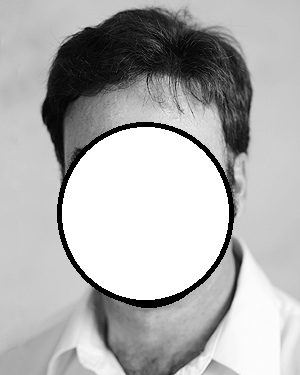
\includegraphics[width=1in,height=1.25in,clip,keepaspectratio]{author1.png}}]{First
        A. Author} received the B.S. and M.S. degrees in aerospace engineering from
    the University of Virginia, Charlottesville, in 2001 and the Ph.D. degree
    in
    mechanical engineering from Drexel University, Philadelphia, PA, in 2008.

    From 2001 to 2004, he was a Research Assistant with the Princeton Plasma
    Physics Laboratory. Since 2009, he has been an Assistant Professor with the
    Mechanical Engineering Department, Texas A{\&}M University, College
    Station.
    He is the author of three books, more than 150 articles, and more than 70
    inventions. His research interests include high-pressure and high-density
    nonthermal plasma discharge processes and applications, microscale plasma
    discharges, discharges in liquids, spectroscopic diagnostics, plasma
    propulsion, and innovation plasma applications. He is an Associate Editor
    of
    the journal \emph{Earth, Moon, Planets}, and holds two patents.

    Dr. Author was a recipient of the International Association of Geomagnetism
    and Aeronomy Young Scientist Award for Excellence in 2008, and the IEEE
    Electromagnetic Compatibility Society Best Symposium Paper Award in 2011.
\end{IEEEbiography}

\begin{IEEEbiography}[{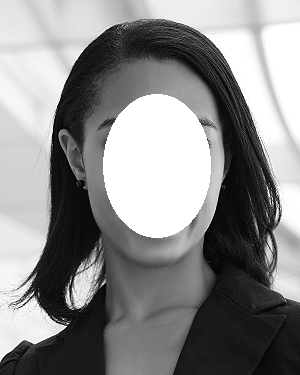
\includegraphics[width=1in,height=1.25in,clip,keepaspectratio]{author2.png}}]{Second
        B. Author} (M'76--SM'81--F'87) and all authors may include
    biographies. Biographies are often not included in conference-related
    papers. This author became a Member (M) of IEEE in 1976, a Senior
    Member (SM) in 1981, and a Fellow (F) in 1987. The first paragraph may
    contain a place and/or date of birth (list place, then date). Next,
    the author's educational background is listed. The degrees should be
    listed with type of degree in what field, which institution, city,
    state, and country, and year the degree was earned. The author's major
    field of study should be lower-cased.

    The second paragraph uses the pronoun of the person (he or she) and not the
    author's last name. It lists military and work experience, including summer
    and fellowship jobs. Job titles are capitalized. The current job must have
    a
    location; previous positions may be listed
    without one. Information concerning previous publications may be included.
    Try not to list more than three books or published articles. The format for
    listing publishers of a book within the biography is: title of book
    (publisher name, year) similar to a reference. Current and previous
    research
    interests end the paragraph.

    The third paragraph begins with the author's
    title and last name (e.g., Dr.\ Smith, Prof.\ Jones, Mr.\ Kajor, Ms.\
    Hunter).
    List any memberships in professional societies other than the IEEE.
    Finally,
    list any awards and work for IEEE committees and publications. If a
    photograph is provided, it should be of good quality, and
    professional-looking. Following are two examples of an author's biography.
\end{IEEEbiography}

\newpage

%If you do not have or do not want to include a photo, you can use IEEEbiographynophoto as shown below:

\begin{IEEEbiographynophoto}{Third C. Author, Jr.} (M'87) received the B.S.
    degree in mechanical
    engineering from National Chung Cheng University, Chiayi, Taiwan, in 2004
    and the M.S. degree in mechanical engineering from National Tsing Hua
    University, Hsinchu, Taiwan, in 2006. He is currently pursuing the Ph.D.
    degree in mechanical engineering at Texas A{\&}M University, College
    Station, TX, USA.

    From 2008 to 2009, he was a Research Assistant with the Institute of
    Physics, Academia Sinica, Tapei, Taiwan. His research interest includes the
    development of surface processing and biological/medical treatment
    techniques using nonthermal atmospheric pressure plasmas, fundamental study
    of plasma sources, and fabrication of micro- or nanostructured surfaces.

    Mr. Author's awards and honors include the Frew Fellowship (Australian
    Academy of Science), the I. I. Rabi Prize (APS), the European Frequency and
    Time Forum Award, the Carl Zeiss Research Award, the William F. Meggers
    Award and the Adolph Lomb Medal (OSA).
\end{IEEEbiographynophoto}

\EOD

\end{document}
